% Figure 3: Results Comparison Bar Chart
% This figure shows the performance comparison across datasets using official results

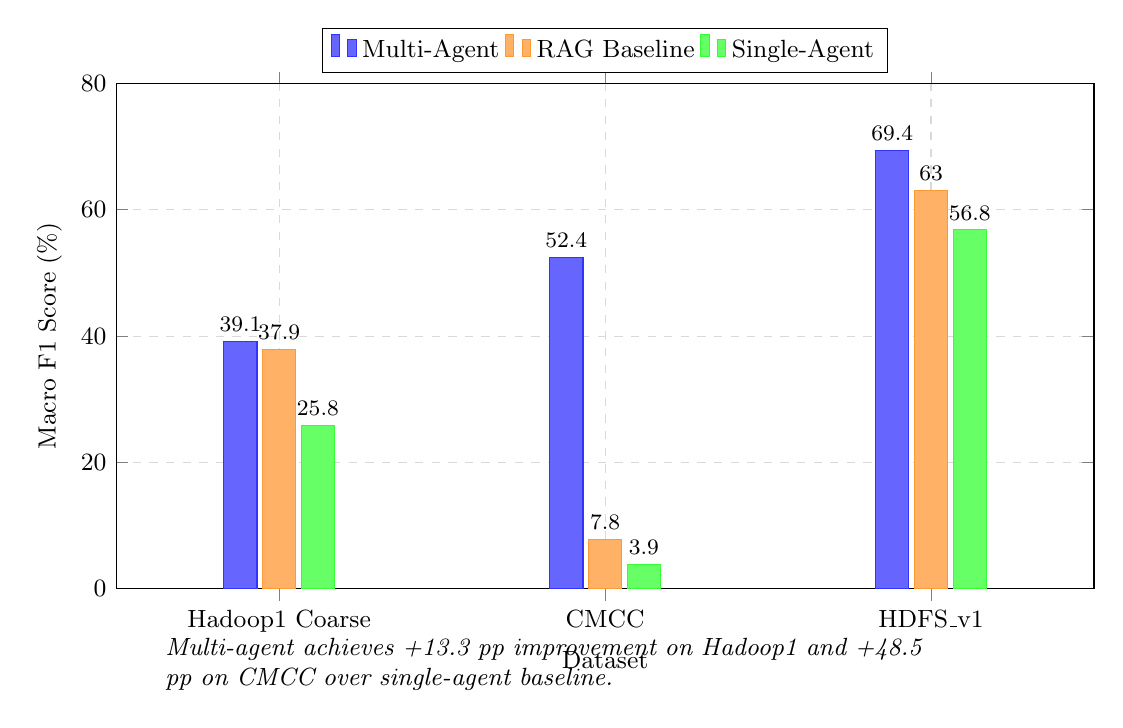
\begin{tikzpicture}
\begin{axis}[
    ybar,
    bar width=12pt,
    width=14cm,
    height=8cm,
    ylabel={Macro F1 Score (\%)},
    xlabel={Dataset},
    ymin=0,
    ymax=80,
    xtick=data,
    symbolic x coords={Hadoop1 Coarse, CMCC, HDFS\_v1},
    legend style={at={(0.5,1.02)}, anchor=south, legend columns=3, font=\small},
    nodes near coords,
    nodes near coords align={vertical},
    every node near coord/.append style={font=\footnotesize},
    enlarge x limits=0.25,
    grid=major,
    grid style={dashed, gray!30},
    tick label style={font=\small},
    label style={font=\small},
]

% Multi-Agent results (official)
\addplot[fill=blue!60, draw=blue!80] coordinates {
    (Hadoop1 Coarse, 39.1)
    (CMCC, 52.4)
    (HDFS\_v1, 69.4)
};

% RAG Baseline results (official)
\addplot[fill=orange!60, draw=orange!80] coordinates {
    (Hadoop1 Coarse, 37.9)
    (CMCC, 7.8)
    (HDFS\_v1, 63.0)
};

% Single-Agent results (official)
\addplot[fill=green!60, draw=green!80] coordinates {
    (Hadoop1 Coarse, 25.8)
    (CMCC, 3.9)
    (HDFS\_v1, 56.8)
};

\legend{Multi-Agent, RAG Baseline, Single-Agent}

\end{axis}

% Annotation for key finding
\node[anchor=north west, font=\small\itshape, text width=10cm] at (0.5,-0.5) {
    Multi-agent achieves +13.3 pp improvement on Hadoop1 and +48.5 pp on CMCC over single-agent baseline.
};

\end{tikzpicture}
